\documentclass{report}
\usepackage[english]{babel}
\usepackage{illcmolthesis}
\usepackage{microtype}
\usepackage{amsmath,amssymb}
\usepackage{amsthm}
\usepackage[round, authoryear]{natbib}
\usepackage[all]{xy}
\usepackage{array}
\usepackage{graphicx}
\usepackage{framed}
\usepackage{enumerate}
\usepackage{qtree}
\usepackage{mdframed}
\usepackage{tikz}
\usepackage{multirow}
\usepackage{pgfplots}
\pgfplotsset{compat = newest}
\usepackage{tikz-dependency}
\usetikzlibrary{matrix}
\usepackage{xfrac}
\usepackage{algorithmic}
\usepackage{pdfpages}
\usepackage{algorithm}
\usepackage{float}
\usepackage[OT2,T1]{fontenc}
\usepackage{hyperref}
%\usepackage[a4paper]{geometry}
\newcommand\textcyr[1]{{\fontencoding{OT2}\fontfamily{wncyr}\selectfont #1}}
\newcommand{\myparagraph}[1]{\paragraph{#1}\mbox{}\\}
\bibliographystyle{plainnat}
\renewcommand\topfraction{0.85}
\renewcommand\bottomfraction{0.85}
\renewcommand\textfraction{0.1}
\renewcommand\floatpagefraction{0.85}

%Define theorem style for definition and metric
\newtheoremstyle{break}  % follow `plain` defaults but change HEADSPACE.
  {\topsep}   % ABOVESPACE
  {15pt}   % BELOWSPACE
  {\itshape}  % BODYFONT
  {0pt}       % INDENT (empty value is the same as 0pt)
  {\bfseries} % HEADFONT
  {.}         % HEADPUNCT
  {\newline}  % HEADSPACE. `plain` default: {5pt plus 1pt minus 1pt}
  {}          % CUSTOM-HEAD-SPEC

\theoremstyle{break}
\newtheorem{metric}{Metric}
\newtheorem{notion}{Notion}
\newtheorem{definition}{Definition}
\def\citepos#1{\citeauthor{#1}'s (\citeyear{#1})}

%Define new float environment for tables that is boxed
\floatstyle{boxed}
\newfloat{tab}{tbp}{lop}
\floatname{tab}{Table}


\begin{document}

\chapter{A new empirical Investigation of Compositionality}

In the previous chapter we have motivated the need for an empirical analysis of compositional translation that combines bilingual information from translation data with monolingual syntactic information produced by a parser. We have introduced alignments and alignment trees, the main ingredients for such a datadriven analysis of compositionality, as well a dependency parses, the monolingual grammar formalism we will use. In this chapter, we will describe the research conducted in this paper, and motivate the explain the procedures that we used. 

We will start this chapter by stating explicitly what the goals of our investigation are, and how we hope to achieve them (Section \ref{sec:goals}). In Section \ref{sec:assumptions}, we will explicate the assumptions that are made in our research (and in empirical research based on real life datasets in general). In Sections \ref{sec:trans_structures} and \ref{sec:deps}, we will revisit the two main ingredients for our empirical analysis, alignment trees and dependency parses, respectively. We will discuss, in case of the former, which subset we are considering, and to how to generate this subset, and how to both alignment trees and dependency parses can be represented. In .... MAAK AF!!




\section{Goals}
\label{sec:goals}

The goals of this thesis are two fold. Firstly, we want evaluate dependencies from a bilingual perspective. That is, we will investigate how well the structure prescribed by a dependency parse coheres with bilingual intuitions, and what the main bottlenecks are. Such an analysis blablabla

Secondly, we want to see if dependency parses can be useful in creating a compositional translation system. This question is related to the former question, as .... and the complexity of determining its answer depends on the answer of the first question. If dependency structures cohere with 

In this thesis, we hope to address the 
With which we address two questions: is compositional translation a reasonable strategy for translation of natural languages, and can we use monolingual syntax to support 

It seems, that a compositional system of meaning for. blabla, should look like a monolingual compositional system.. 

- how well do dependency parses represent monolinguistic structure from a bilingual perspective
- can we use this information to design a compositional grammar

\begin{enumerate}
\item Can translation of natural language be treated compositionally?
\item in particular: can monolingual syntax be helpful
\item $\Rightarrow$ find evidence in real data
\item more
\end{enumerate}


For such a study, an idiomatic expression or a strange phenomenon sitting in a corner of language is no evidence against compositionality, rather, we want to know how many phenomena and expressions are sitting in this corner, and if we can add all these phenomena and expressions to a compositional grammar without loosing the feeling that overall translations were compositional.

\begin{figure}[!ht]
\centering
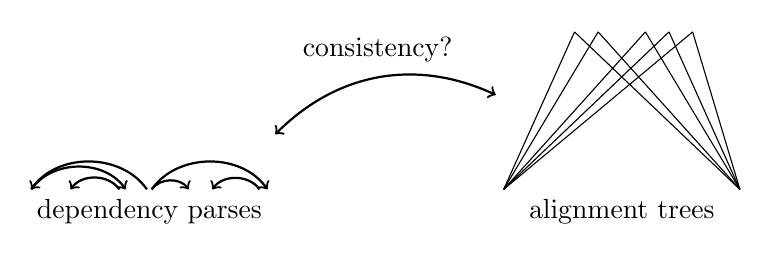
\begin{tikzpicture}

\coordinate (ss) at (1.5,0);
\node [below] at (ss) {dependency parses};

\draw[->,bend right = 55,thick] (1.47,0) to (0,0);
\draw[->,bend left = 55, thick] (1.53,0) to (3,0);
\draw[->,bend left = 55, thick] (0.0,0) to (1.2,0);
\draw[->,bend right = 55,thick] (1.12,0) to (0.5,0);
\draw[->,bend left = 55, thick] (1.53,0) to (2.0,0);
\draw[->,bend right = 55,thick] (2.9,0) to (2.3,0);

\coordinate (ts) at (7.5,0);
\node [below] at (ts) {alignment trees};

%\draw (6,0) -- (0.6,2) (9,0) -- (6.6,2);
\draw (6,0) -- (6.9,2) (9,0) -- (6.9,2);
\draw (6,0) -- (7.2,2) (9,0) -- (7.2,2);
%\draw (6,0) -- (7.5,2) (9,0) -- (7.5,2);
\draw (6,0) -- (7.8,2) (9,0) -- (7.8,2);
\draw (6,0) -- (8.1,2) (9,0) -- (8.1,2);
\draw (6,0) -- (8.4,2) (9,0) -- (8.4,2);

\coordinate (startarrow) at (3.1,0.7);
\coordinate (endarrow) at (5.9,1.2);
\node (t) at (4.4,1.5) [above]{consistency?};

\draw[<->,bend left =35, thick] (startarrow) to (endarrow);

\end{tikzpicture}
\caption{New situations: finding consistency between dependency parses and compositional translation structures}\label{fig:depshats}
\end{figure}

\section{Foundations of Empirical Studies}
\label{sec:assumptions}

The analysis of compositionality presented in this thesis is based on real data, that are not always perfect. When training MT models, infrequent mistakes in the data are generally not problematic, as they will receive a low probability. The same cannot be said for empirical analysis, were mistakes in the data will almost always harm the outcome. It therefore seems sensible to see empirical analysis as providing an upper- or lower bound (depending on the context) rather than an exact number. To appreciate empirical research, it is important to to know about the factors that influence the results, and the simplifying assumptions that are made to make it possible. In this section, we will discus these factors and assumptions, some of which may sound obvious, to provide a complete picture of the foundations of empirical studies.

\subsection{Correctness of the Translation Data}

Empirical analyses based on parallel corpora with text that are each others translation, rely heavily on the correctness of the data in these these corpora. As these parallel texts were not designed as data for translation models, they might not be perfectly suitable for this purpose. There are three bottlenecks:

\subsubsection{Sentence level alignment.}
Aligning corpora on the sentence level is not as simple as it might seem. Texts are not always translated sentence by sentence. Short sentences may be merged or long ones broken up, and in some languages sentence delimiters do not really exist \citep[p.55]{koehn2008statistical}. However, the techniques for sentence alignment are very good, and as the languages we are considering \textit{do} have clear sentence delimiters it seems very reasonable to assume that the sentences in the corpora are correctly aligned.

\subsubsection{Correctness of translation.}
The translations of the sentences are produced by humans, who sometimes make mistakes. To use the corpora, we have to assume that the aligned sentences are good translations of each other.

\subsubsection{Translation is literal.}
One English sentence often has many translations in another language, as similar meanings can be expressed in multiple ways.\footnote{In fact, considering only one target translation can also be seen as a simplification made in empirical research, and in MT in general.} For instance `jeg giver dig blomster' is a good Danish translation of `I give you flowers', but so is `jeg giver blomster til dig' (and the amount of rephrasing in this example is even rather minimal). Especially when one text is not a direct translation of the other text, but the two are, for instance, just separate reports of the same event, it might happen that sentences do have the same meaning, but are not very similar in form. In our analysis, we will assume that at least the vast majority of the translations in the corpora are rather literal.
 
\subsection{Correctness Word Alignments}

In empirical analyses, as well as MT-models, word-alignments are used to establish translational correspondences, and are thus of crucial importance. Unfortunately, automatic alignments are not always as good as we want them to be \citep{och2000improved}. MT-models generally do not suffer much from this fact, because the number of untrue alignment links is dwarfed by the number that is correct. For empirical research, false alignment links are quite problematic, as even one wrong link can have a huge effect on the space of possible translation trees. An option is to use one of the few manually aligned corpora, but given their small size they are not suitable to draw conclusions about larger parts of language.

\subsection{Correctness Dependency Parses}

To determine the dependency structures of the sentences in the corpus, an efficient fully automated dependency parser is needed.  For English, high quality dependency parses are available \citep{cer2010parsing}, but the parses they produce are not perfect, which can be problematic for an empirical analysis.



\section{Translation Structures}

The bilingual part of our analysis is constituted by a subset of all alignment trees as described in \ref{subsec:alignment_trees}. We will consider all alignment trees that are \textit{maximally compositional} (they describe a translation with a maximal number of rules). This subset was previously defined in \cite{simaan2013hats}, we will follow their notation and call them Hierarchical Alignment Trees (HATs). In \cite{simaan2013hats}, the nodes of the HATs are augmented with operators that describe how its children should be permuted to obtain the corresponding target side tree. We will not consider these operators in this thesis, and the term `HAT' will thus refer to a skeleton of a HAT, rather than its full version. In this section, we will give an intuitive description of a HAT skeleton, that will help us to motivate our choice for this subset, and we will ..  MAAK AF!

\subsection{Motivation}

A HAT describes a maximally compositional translation of a sentence, given its alignment, and is characterised by the following properties:\begin{enumerate}
\item A HAT is a projective tree whose leaf nodes form a sentence.
\item A HAT describes a compositional translation of the sentence constituted by its leaf nodes.
\item All non-terminal nodes dominate a translation admissible sequences, while sibling non-terminal nodes together constitute a translation admissible sequence.
\item A node in a HAT can have both non-terminal and terminal child nodes at the same time.
\item All nodes in a HAT expand into a minimal number of children.
\end{enumerate}

\noindent Maximum compositionality gives HATs several attractive properties, which we will discuss in this subsection.

\subsubsection{Computational}
There is a clear computational advantage to considering only minimally branching trees. Not only does it significantly reduces the space of trees to be considered - the example sentence previously used in Section \label{sec:comp_structures} for explaining alignment trees\footnote{Sentence pair: (`My dog also likes eating sausages', `Mijn hond houdt ook van worstjes eten')\\Set-permutation: $\langle \{0\}, \{1\}, \{3\}, \{2,4\}, \{6\}, \{5\}\rangle$. } has 44 alignment trees, but only 5 of them are minimally branching - it also simplifies parsing, as the lower-rank rules that can be extracted from minimally branching trees can be more efficiently treated by parsing algorithms.

\subsubsection{Theoretical}

Of course, such computational considerations are less important for an empirical analysis (although even for empirical analysis computational requirements should match the reality). However, also theoretically HAT skeletons are very attractive, which we will explicate in the following paragraphs.

\paragraph{Compositionality} Considering only minimally branching trees secures that the system we are studying is in fact compositional. The set of all alignment trees contains many flat trees, that can strictly speaking be seen as compositional (as compositionality is highly underspecified in this respect), but do not capture the recursive and systematic nature of language. A compostional system containing a separate rule for almost every sentence that specifies how its meaning can be derived from \textit{all of its words} does certainly not correspond with human intuitions about compositionality, not to mention the fact that such a system should have an infinite number of rules to cover the entire language, considering only minimally branching trees sovles this problem.

\paragraph{Generalisation} Considering only expansions that are maximally compositional maximises the chance that generalisation to new data is possible: a rule that specifies how a type of argument can be combined with a type of predicate is more useful than a rule specifying how the argument `I' can be combined with the predicate `like'. Minimum depth expansions are more probable to be applicable in new situations. 

Figure \ref{fig:nepas} shows how French negation, often mentioned as problematic for structure based systems, is accounted for with a HAT skeleton. The translation tree shows that `I dont like' is the translation of `Je n'aime pas', but also contains the information that `don't' is phrasally translated as `ne ... pas'. Removing the negation in the English sentence results in the grammatical English sentence `I like cars', removing its translation equivalent in the France sentence in its (almost) grammatical `Je aime les voitures'. 

\begin{figure}[!ht]
\centering
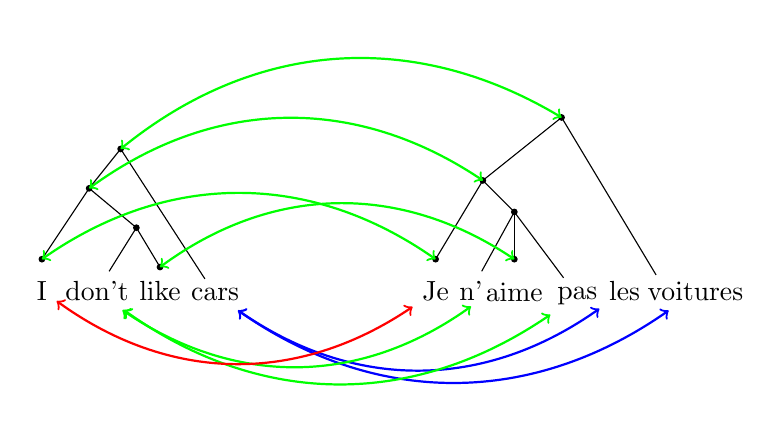
\begin{tikzpicture}
\draw node (I) at (0,0) {I};
\draw node (dont) at (0.7,0) {don't};
\draw node (like) at (1.5,0) {like};
\draw node (cars) at (2.2,-0.05) {cars};

\draw node (Je) at (5.0,0) {Je};
\draw node (n) at (5.45,0) {n'};
\draw node (aime) at (6.0,-0.02) {aime};
\draw node (pas) at (6.8,-0.07) {pas};
\draw node (les) at (7.4,0) {les};
\draw node (voitures) at (8.3,-0.01) {voitures};

\coordinate (Je_) at (5.0,0.4);
\coordinate (like_) at (1.5,0.3);
\coordinate (I_) at (0,0.4);
\coordinate (aime_) at (6.0,0.4);
\coordinate (naimepas) at (6.0,1);
\coordinate (dontlike) at (1.2,0.8);
\coordinate (Idontlike) at (0.6,1.3);
\coordinate (Jenaimepas) at (5.6,1.4);
\coordinate (lesvoitures) at (7.8,0.2);
\coordinate (all) at (1,1.8);
\coordinate (tout) at (6.6,2.2);
\coordinate (n_) at (5.45,-0.2);

\foreach \coordinate in {dontlike, like_, I_, Je_, aime_, Idontlike, all, tout, Jenaimepas, naimepas}
	\filldraw (\coordinate) circle (0.035);

\foreach \from/\to in {naimepas/aime_, naimepas/n, naimepas/pas, dontlike/like_, dontlike/dont, Idontlike/I_, Idontlike/dontlike, all/Idontlike, all/cars, Jenaimepas/Je_, Jenaimepas/naimepas, tout/Jenaimepas, tout/lesvoitures}
	\draw (\from) -- (\to);

\foreach \from/\to in {cars/voitures, cars/les}
	\draw[<->, bend left = -35, thick, blue] (\from) to (\to);

\foreach \from/\to in {dont/n_, dont/pas, tout/all, Jenaimepas/Idontlike, aime_/like_, Je_/I_}
	\draw[<->, bend left = -35, thick, green] (\from) to (\to);

\draw[<->, bend left = -35, thick, red] (I) to (Je);

\end{tikzpicture}
\caption{Translation of negation, French-English}\label{fig:nepas}
\end{figure} 

\paragraph{Preservation of structure of phrasal translations}

An advantage that overlaps with the two previously mentioned advantages, but is worth noting nevertheless, is the fact that structure of phrasally translated sequences is preserved, if possible. As the rest of the tree, sequences of words will be translated directly only if they do not have a deeper structure according to the translation data. In many phrase-based translation systems, including the successful hierarchical phrase based system proposed by \cite{chiang2007hierarchical}, the underlying system of sequences that are translated phrasally gets lost in the process, whereby the system misses an opportunity to detect a pattern. HAT skeletons fully exploit recursiveness, also in idiomatic and phrasal translations. We will revisit an example containing syntactic translation to illustrate how a structural treatment of phrasal translation is helpful.

In Russian, `X has Y` is (communistically) translated as `with X is Y', the object in English is thus the subject in Russian. Figure \ref{fig:russian} shows how this is dealt with in a translation structure. Due to the structural treatment of the phrasal translation, this translation tree is easily extendible to longer sentences with the same construction. By expanding the non-terminal nodes it can also capture sentences like `the girl with the long blond hair has a very old car with broken windows'.

\begin{figure}[!ht]
\centering

\begin{tikzpicture}

\draw node (the) at (0,0.02) {The};
\draw node (girl) at (0.75,0) {girl};
\draw node (has) at (1.4,0.04) {has};
\draw node (a) at (1.9,0) {a};
\draw node (car) at (2.4,0) {car};
\draw node (y) at (4,0) {\textcyr{u}};
\draw node (girlr) at (4.9,-0.02) {\textcyr{devuxki}};
\draw node (is) at (6.1,0.02) {\textcyr{est\char126}};
\draw node (carr) at (7.5,0.04) {\textcyr{avtomobil\char126}};

\coordinate (thegirl) at (0.4,0.6);
\coordinate (acar) at (2.1,0.6);
\coordinate (thegirlhas) at (0.8,1);
\coordinate (all) at (1.4,1.5);
\coordinate (carr_) at (7.5, 0.3);
\coordinate (girlr_) at (4.9,0.3);
\coordinate (girlhas) at (4.9,0.8);
\coordinate (allr) at (5.9, 1.2);


\foreach \coordinate in {thegirl, acar, thegirlhas,all,carr_, girlr_, girlhas, allr}
	\filldraw (\coordinate) circle (0.035);

\foreach \from/\to in {thegirl/girl, thegirl/the, acar/a, acar/car, thegirlhas/thegirl, thegirlhas/has, all/thegirlhas, all/acar, girlhas/girlr_, girlhas/y, girlhas/is, allr/girlhas, allr/carr_}
	\draw (\from) -- (\to);

\foreach \from/\to in {the/girlr, girl/girlr}
	\draw[<->, bend left = -35, thick, blue] (\from) to (\to);

\foreach \from/\to in {has/y, has/is, allr/all, girlhas/thegirlhas, carr_/acar, girlr_/thegirl}
	\draw[<->, bend left = -35, thick, green] (\from) to (\to);

\foreach \from/\to in {a/carr, car/carr}
	\draw[<->, bend left = -35, thick, red] (\from) to (\to);

\end{tikzpicture}
\caption{Translation of possession, Russian-English}\label{fig:russian}
\end{figure}


\subsubsection{Critical Note}

Intuitively, \textit{maximal} compositionality is sometimes a bit strict. When constructing a sentence that has an predicate with two arguments, it is linguistically not always plausible to assume that the predicate is combined with the arguments one by one. In translation, this issue issue is enhanced by the fact that arguments of a predicate may not be in the same order for different languages. A HAT describing a translation in which this happens is forced to combine the arguments with each other before combining them with the predicate. Although these issues do not influence the generative capacity of the system, their treatment may sometimes seem counter intuitive.


\subsection{Representation}

To study HATs, we need to be able to generate the HAT skeletons for every sentence. Generating and storing all trees separately would be both time and space consuming, and would impede a flexible search through them. Hence, a suitable representation of the set of HATs is required. In this thesis, we will represent the set of HATs for a sentence implicitly by a context-free grammar, that describes for every (translation admissible) span of the sentence how it is allowed to split in parts. The nodes are labelled with the spans they dominate. Figure \ref{fig:grammar} provides an example. %Explain the advantages of representing HATs with contextfree grammars?

\begin{figure}[!ht]\begin{framed}
\small{
\begin{tabular}{llllll}
(0-6] $\rightarrow$ (0-1]  (1-6] && (4-6] $\rightarrow$ (4-5]  (5-6] && (0-1] $\rightarrow$ My\\
(0-6] $\rightarrow$ (0-2]  (2-6] && (0-4] $\rightarrow$ (0-1]  (1-4] && (1-2] $\rightarrow$ dog\\
(0-6] $\rightarrow$ (0-4]  (4-6] && (0-4] $\rightarrow$ (0-2]  (2-4] && (2-3] $\rightarrow$ also\\
(1-6] $\rightarrow$ (1-4]  (4-6] && (1-4] $\rightarrow$ (1-2]  (2-4] && (4-5] $\rightarrow$ eating\\
(1-6] $\rightarrow$ (1-2]  (2-6] && (0-2] $\rightarrow$ (0-1]  (1-2] && (5-6] $\rightarrow$ sausages\\
(2-6] $\rightarrow$ (2-4]  (4-6] && (2-4] $\rightarrow$ (2-3] likes\\
\end{tabular}
\caption{The grammar generating the translation tree forest for the sentence
`My dog also likes eating sausages', with set-permutation $\langle _0\{0\}_1,~ _1\{1\}_2,~ _2\{3\}_3,~ _3\{2,4\}_4, ~_4\{6\}_5,~ _5\{5\}_6\rangle$ would be (the subscripts indicating the span annotation, which is left exclusive and right inclusive)}\label{fig:grammar}
}
\end{framed}
\end{figure}

The allowed expansions were found with an algorithm similar to \citepos{dijkstra1959note} shortest path algorithm (Algorithm \ref{alg:shortest paths}), that was adapted to be more efficient given the extra knowledge of the alignment graph.

\begin{algorithm}[!ht]
\caption{Shortest Paths}\label{alg:shortest paths}
\begin{algorithmic}
\STATE \textbf{Input:} A graph $G = (V,E)$ describing an alignment and two vertices $i$ and $j$ for which $(i,j)\in E$ is true.
\STATE \textbf{Output:} All non-trivial shortest paths from $i$ to $j$
\STATE \textit{\#Initialization}
\STATE visited = $\emptyset$, depth = $0$, paths = $\{j\}$
\STATE $\forall n\in\mathbb{N}:$ reachable(n) = $\emptyset$; reachable($0$) = $\{j\}$
\STATE depth\_finished = False
\STATE \textit{\# Start backwards search through graph}
\WHILE{not depth\_finished or $i\notin$ visited}
	\WHILE{reachable(depth) $\neq\emptyset$}
		\STATE depth\_finished $\leftarrow$ False
		\STATE current\_node $\leftarrow N$ an arbitrary element $v$ from reachable(depth)
		\STATE reachable(depth) $\leftarrow$ reachable(depth) $-$ $\{$current\_node$\}$
		\FOR{ ($l$,current\_node) $\in E$}
			\IF{$l\notin $visited $\cup$ reachable(depth) \AND depth $\neq 0$}
				\STATE reachable(depth+1) $\leftarrow$ reachable(depth+1) $\cup$ $\{l\}$
				\FOR{path (current\_node,\ldots, $j) \in$ paths}
					\STATE path $\leftarrow$ ($l$,current\_node,\ldots, $j)$
				\ENDFOR
			\ENDIF
		\STATE visited $\leftarrow$ visited $\cup$ $\{l\}$
		\ENDFOR
	\STATE depth\_finished $\leftarrow$ True
	\STATE depth $\leftarrow$ depth+1
	\ENDWHILE
\ENDWHILE
\STATE \textbf{Return} paths
\end{algorithmic}
\end{algorithm}


\section{Dependency parses}

The monolinugal part in our analysis consists of information about the dependency structure of a sentence. Following common practice, in this thesis it is assumed that this dependency structure satisfies the following two conditions:\begin{enumerate}
\item When seen as a relation, $D$ constitutes a single-headed a-cyclic graph in which the words in $s$ are the nodes. (tree-constraint)
\item When the words are placed in the original order, the branches of the dependency tree do not cross. (projectivity)
\end{enumerate}

As we have already defined dependency parses in Section \ref{sec:dep_parse}, we will not do this again. We will, however, explicate how we represent and generate dependency parses.

\subsection{Representation}

We will represent a dependency parse as a set of relations, as is expressed in the following definition:\footnote{Note that this definition is different from the definition given in \ref{sec:dep_parse}, but expresses the same type of object.}

\begin{definition}[Dependency structure]
A dependency structure of a sentence $s = w_0\cdots w_n$ is a set of dependencies $D = \{ (i,j) |$ there is a dependency arrow from word $w_i$ to word $w_j \}$. 
\end{definition}

Formally, dependency grammars are not interpreted as compositional grammars, as they do not postulate the existence of non-terminal syntactic categories and therefore do not explicitly specify how a sentence was built up from its parts. However, dependency graphs do give rise to an hierarchical structure, that specifies from which smaller parts the sentence was composed. For instance, the dependency graph depicted in Figure \ref{fig:deptree1} tells us that `likes' is the head word of the sentence, and that the sentence is composed of 4 parts: the head `likes', its modifier `also', its noun subject whose head is `dog' and the open clausal complement whose head is `eating'. The complement and subject are further divisible in `My' and `dog', and `eating' and `sausage', respectively. As the tree is projective, all parts are continuous. Also the graph in Figure \ref{fig:depgraph} we saw earlier prescribes an hierarchical structure: it is composed of the subject `I', the headword `know', and the phrase headed by `liet', that is in its turn built up from its head `liet', `dat', `hij' and the discontinous phrase `me winnen'. Such an hierarchical structure can not be captured by a phrase structure grammar.

\begin{figure}[!h]\label{fig:deptree1}
\centering
\begin{dependency}[theme=simple]%[hide label]
\begin{deptext}[column sep=.5cm, row sep=.1ex]
%PRP\$ \& NN \& RB \&[.5cm] VBZ \& VBG \& NN \\
My \& dog \& also \& likes \& eating \& sausage \\
\end{deptext}
\deproot{4}{}
\depedge{2}{1}{poss}
\depedge{4}{2}{nsubj}
\depedge{4}{3}{xvmod}
\depedge{4}{5}{xcomp}
\depedge{5}{6}{dobj}
\end{dependency}
\caption{Stanford Dependency Tree}\ref{fig:deptree}
\end{figure}

\subsection{Generation}

To assign dependency structures to sentences, we used the Stanford Dependency Parser, that can be downloaded from their website, as well as used online  \citep{de2006generating}. The parser provides 5 variants of a typed dependency representation, of which the most basic one corresponds to the earlier imposed conditions on dependency structures. A picture of a dependency parse that was generated by the parser is depicted in Figure \ref{fig:deptree}.

Unfortunately, the dependency parser used \citep{de2006generating} does not cover all tokens of the input sentences, as dependency relations between words and punctuation are not present in the Stanford Dependency Representation. The resulting dependency trees do thus not always cover the entire sentence.


\section{Dependency Grammars from a bilingual perspective.}

In this section, we will discuss how the consistency between dependency grammars and translation data can be measured.

\subsection{Scoring an Alignment Tree}

Quantifying the consistency between a dependency tree and an alignment is not trivial. When a dependency tree prescribes a parts that are all parts according to the alignment, there is no dubiety: such an alignment should get an optimal score. If this is not the case, it is less clear, as there are multiple things that should be taken into account. Not only should the measure of consistency be based on whether the head and its dependent are both phrases according to the alignment, they should also be combined in a reasonable fashion.

To give an abstract example, consider the following dependency parse and alignment trees:

\begin{figure}[ht!]
\centering
{\footnotesize
\begin{tabular}{m{3.5cm}m{2.3cm}m{2.3cm}m{2.3cm}}
\begin{dependency}[theme=simple]%[hide label]
\begin{deptext}[column sep=.5cm, row sep=.1ex]
A \& B \& C \& D \\
\end{deptext}
\depedge{4}{3}{}
\depedge{4}{2}{}
\depedge{2}{1}{}
\end{dependency} \qtreecenterfalse & \Tree [ [ [ A B ] C ] D ] & \Tree [ [ A B ] [ C D ] ] & \Tree [ [ A B ] C D ]
\end{tabular}}
\end{figure}

All the parts that exist in the dependency tree also exist in all alignment trees. The third alignment tree is obviously most similar to the dependency parse, as it prescribes the same compositional structure, and uses the same number of rules. However, the first and second alignment tree are indistinguishable if only the number of correct (and possibly incorrect) nodes is considered, as they both contain two correct, and one incorrect node. However, the second alignment tree seems more in line with the dependency parse than the first one, as it does not only prescribes that A should be combined with B into a new part, but also that C and D are combined in the same stage.

The analysis of the example provided a new insight, as it seems, alignment trees and dependency parses are intuitively compatible if the relations in the dependency parse are respected by the alignment tree, and the score of an alignment should be proportional with what percentage of all dependency relations is respected by it. An alignment will then receive of its alignment trees that scores highest.

\subsection{Consistency of Dependency Relations}

Whether a dependency relation is respected by an alignment tree can be defined in different fashions.

\subsubsection{Direct Consistency}

Consistency of dependency relations can be define rather directly, by saying that a dependency relation is consistent with an alignment tree if both the head and the phrase headed by its argument are siblings in the tree, which is expressed in the following definition:

\begin{definition}[Direct Consistency]\label{def:depHAT}
Let $s = w_1 w_2 \dots w_n$ be a sentence, and $D = \{ (i,j) |$ there is a dependency arrow from word $w_i$ to word $w_j \}$ a set of dependencies describing a dependency tree for $s$. Let span($j$) be the range $[m,n]$ in which $m$ and $n$ are the maximum and minimum position that can be reached from $w_j$ by following the directed dependency arrows, respectively. A dependency relation $(i,j)$ is said to be respected by an alignment tree $T$ over $s$ if and only if there is a node in $T$ of which both $[i,i]$ and span($j$) are children.
\end{definition}

Under this definition of consistency, the first alignment tree in the previous example would receive a score of 1/3, the second alignment tree would receive a score of 2/3, and the third alignment tree a score of 3/3. Which seems to correspond with their adequacy of describing the dependency structure.

\subsubsection{Deeper Consistency}

We have previously mentioned, that assuming maximal compositionality is not necessarily in line with linguistic intuitions. Dependency parses are certainly general, but are not constructed to be \textit{maximally} recursive. We will give two examples of sentences that are intuitively compositionally translated, but do not get a maximal score due to this issue.

Firstly, consider the sentence `I give you flowers', and its (word-for-word) translation `Ik geef jou bloemen', with dependency parse:

\begin{figure}[!ht]
\centering
{\small
\begin{tabular}{m{5.5cm}m{5cm}}
\begin{dependency}[theme=simple]%[hide label]
\begin{deptext}[column sep=.5cm, row sep=.1ex]
I \& give \& you \& flowers \\
\end{deptext}
\depedge{2}{1}{subj}
\depedge{2}{3}{iobj}
\depedge{2}{4}{dobj}
\end{dependency} & \qtreecenterfalse \Tree [ I give you flowers ]
\end{tabular}
}
\end{figure}

The tree depicted next to the dependency parse is the only tree that respects all dependency relations. The sentence is very short and the dependency parse therefore very flat. In a tree that respects all relations according to Definition \ref{def:depHAT}, `I', `give', `you', and `flowers' are all siblings, which means the tree depicted next to the dependency parse is the only tree obtaining a maximal score. However, as the sentence is word for word translation, all subsequences are translation admissible, and all HATs will be completely binary. Even though the translation seems intuitively compositional, none of the HATs will receive a score higher than 1/4, because the dependency parse is not maximally branching.

A similar situation arises when two arguments are translated into one which happens, e.g., when arguments are translated as pre- or suffixes, when verbs do not require a subject or when spaces are emitted). Consider for instance the sentence 'Can you give me the salt' and its Italian translation 'puoi passarmi il sale':

\begin{figure}[!ht]
\centering
{\small
\begin{tabular}{m{6.7cm}m{6.7cm}}
\begin{dependency}[theme=simple]%[hide label]
\begin{deptext}[column sep=.5cm, row sep=.1ex]
Can \& you \& give \& me \& the \& salt \\
\end{deptext}
\depedge{3}{1}{aux}
\depedge{3}{2}{nsubj}
\depedge{3}{4}{iobj}
\depedge{6}{5}{det}
\depedge{3}{6}{dobj}
\end{dependency} &
\begin{dependency}[theme=simple]\begin{deptext}[column sep=.5cm, row sep=.1ex]
Puoi \& passarmi \& il \& sale \\
\end{deptext}
\deproot{2}{root+iobj}
\depedge{2}{1}{aux+nsubj}
\depedge{2}{4}{dobj}
\depedge{4}{3}{det}
\end{dependency} 
\end{tabular}
}
\end{figure}

Once again, the predicate-argument structure of the sentence is well preserved. However, the some of the arguments are merged into single words in the italian sentence. Besides the issue raised in the previous paragraph (the dependency structure is not maximally compositional), an additional problem thus arose: except for `me', none of the arguments can combine directly with `give' in an alignment tree, because `give' and `me' are one word in Italian, and will thus form a unit on their own. `Can' and `you' cannot combine with `give' at all, because they are first combined together. The maximum score a HAT of this translation could receive would thus be 2/5, in which only the relations (give, me) and (salt, the) are respected.

To solve such issues, predicates should be able to combine with their arguments in stages (e.g., combine `give' with `you', combine `give you' with `flowers', combine `I' with `give you flowers'). Under this perspective, a dependency relation is respected by a HAT if it is siblings with the head itself, or the head plus arguments the head earlier combined with, which is expressed in the following definition:

\begin{definition}[]\label{def:depHAT2}
Let $s = w_1 w_2 \dots w_n$ be a sentence, and $D = \{ (i,j) |$ there is a dependency arrow from word $w_i$ to word $w_j \}$ a set of dependencies describing a dependency tree for $s$. Let span($j$) be the range $[m,n]$ in which $m$ and $n$ are the maximum and minimum position that can be reached from $w_j$ by following the directed dependency arrows, respectively. Let $(i,j)$ be a dependency relation in $D$, and let $l_1,\ldots,l_n$ and $r_1,\ldots r_k$ be the left and right dependents of $i$, respectively, for which holds that $r_k < j$ or $l_1 > j$. A dependency relation $(i,j)$ is said to be respected by an alignment tree $T$ over $s$ if and only if one of the following three conditions is true: \begin{enumerate}
\item There is a node in $T$ f which both $[i,i]$ and span($j$) are children.
\item $\exists x$  and a node in $T$ of which span($l_x\ldots l_n~i~\ldots r_1 r_k$) and span($j$) are both children.
\item $\exists x$  and a node in $T$ of which span($l_1\ldots l_n~i~r_1\ldots r_x$) and span($j$) are both children.
\end{enumerate} 
\end{definition}

This extension of the definition of consistency between HATs and dependency parses solves the discrepancy between the type of compositionality of HATs and dependency parses only partly. The first example receives a maximal score using this definition, but the second does not, as `can' and `you' can still not combine with give one by one. Definition \ref{def:depHAT2} can also not account for severe reordering of the arguments in translation. However, we believe that extending the definition even further (by for instance allowing the arguments to combine all together first and then with the argument, or with part of the argument), would move away too far from what the dependency parse is in fact encoding. %I am not sure if I should put this in at all?


\paragraph{Remark} As previously mentioned, the Stanford Dependency style does not include punctuation. Where in the first consistency definition this did not really get in the way, it becomes problematic for the second, as tokens that are not involved in any dependency relation can interfere with the definition of consistency. To account for this, we allowed punctuation (or other tokens not processed by the dependency parser) to combine freely with the closest units (of arbitrary size), without them affecting the score.

\subsection{Scoring Alignments}

A alignment will be scored by finding it highest scoring alignment tree, that is recursively defined as follows:

\begin{definition}[Score of an Alignment Tree]
 $s = w_1 w_2 \dots w_n$ be a sentence, and $D = \{ (i,j) |$ there is a dependency arrow from word $w_i$ to word $w_j \}$ a set of dependencies describing a dependency tree for $s$. Let $T$ be an alignment tree of $S$, and let $\mathcal{M}$ be the metric that decides what is needed for a dependency relation to be true in $T$. $M$ is associated with a set containing relations between nodes that make the relations in $D$ true, call this set $D'$. The (unnormalised) score of $H$ with $D$ is now defined as the score of its highest node $N$:

$$
E(N_a,D) = \sum_{c\in C_{N_a}} E(c,D)+ \sum_{c_1\in C_{N_a}} \sum_{c_2\in C_{N_a}} B(c_1,c_2)
$$

\noindent With base case $E(N,D) = 0$, $B(c_1,c_2) = 1$ iff  $(c_1,c_2)\in D'$, and $C_N$ the set of child nodes of $N$.

The score can be normalised by dividing by $|D|$.
\end{definition}

The score of an alignment can now be determined by parsing the corresponding sentence with the grammar that represents its HAT forest of the alignment to find its best HAT. Details on implementation can be found in Appendix \ref{appendix:implementation}.

\section{Bilingual grammars Using Dependency grammars}

Something about EM and training a grammar


\section{Implementation}

The program that was developed for these experiments is available on
\href{https://github.com/dieuwkehupkes/Thesis}{https://github.com/dieuwkehupkes/Thesis}. Appendix \ref{appendix:implementation} provides an extensive documentation for the program, as well as instructions on how to download and use it.

\bibliography{thesisDH}
\end{document}